\documentclass[11pt]{article}
\usepackage[a4paper,margin=1in]{geometry}
\usepackage{graphicx}
\usepackage{booktabs}
\usepackage{amsmath}
\usepackage{hyperref}
\usepackage{authblk}
\usepackage{caption}

\title{Weather Intelligence and Climate Decision Support Platform: \\
An AI System for Southwest Monsoon Precipitation Forecasting Integrating \\
Machine Learning, Deep Learning, Computer Vision, and Generative AI Agents}

\author[1]{Purva Tayade}
\affil[1]{Generative AI Research Internship, MacroEdtech}
\date{August 2026}

\begin{document}

\maketitle

\begin{abstract}
The Southwest Monsoon is the dominant weather system governing India's agriculture, water resources, food security, and disaster management. This paper presents an end-to-end, open-source AI system for forecasting monsoon-season precipitation and temperature for Mumbai, India, combining classical machine learning, time-series, and deep learning models with a Retrieval-Augmented Generation (RAG) and agentic Large Language Model (LLM) layer. Ten years (2015--2025) of daily meteorological data were collected from the Open-Meteo Archive API and cross-validated against NASA POWER. Seven forecasting approaches were compared -- Linear Regression, Random Forest, XGBoost, LightGBM, Prophet, SARIMAX, and a Long Short-Term Memory (LSTM) network -- with Random Forest achieving the best precipitation forecasting performance (MAE = 3.44~mm, R\textsuperscript{2} = 0.669). Model behaviour was explained using both SHAP and LIME, which independently identified prior-day precipitation and relative humidity as the dominant predictors. The prediction engine was deployed as a FastAPI/Streamlit application and extended into a Generative AI assistant using a ChromaDB vector store, a LangGraph tool-calling agent with conversation memory, and a genuine Model Context Protocol (MCP) server-client integration. Honest limitations are reported throughout, including systematic disagreement between data sources, model under-prediction of extreme rainfall events, tool-calling reliability differences between small and large open-weight LLMs, and an unresolved local Docker deployment blocker.
\end{abstract}

\section{Introduction}

\subsection{Problem Statement}
The Southwest Monsoon is the primary weather system influencing India's agriculture, water resources, food security, energy production, transportation, and disaster management. Variability in monsoon onset, intensity, duration, and spatial distribution frequently causes floods, droughts, landslides, crop losses, and infrastructure damage. Reliable forecasting and climate intelligence tools are therefore critical for disaster risk mitigation and climate adaptation.

\subsection{Objective}
This work designs, develops, and evaluates an open-source AI-powered Weather Intelligence and Climate Decision Support Platform for the Indian Southwest Monsoon system, integrating machine learning, deep learning, time-series forecasting, computer vision/remote sensing, and a Generative AI (RAG + agentic) layer, using only free and open-source tools, models, and publicly available data.

\subsection{Literature Review}
Indian Summer Monsoon Rainfall (ISMR) forecasting has a long history of statistical and, more recently, machine-learning approaches. Kumar et al.~\cite{kumar2025ann} propose an artificial neural network with a stacked autoencoder over ten climate parameters to forecast ISMR, achieving a Pearson correlation of 0.829 between observed and forecast rainfall, and note that traditional statistical methods have historically struggled to provide precise quantitative forecasts at fine spatial resolution. Dash et al.~\cite{dash2018comparison} compare iterative and non-iterative machine learning approaches for ISMR prediction, finding that ensemble and iterative learning strategies improve on classical regression baselines. These works motivate the feature-engineering and model-comparison approach taken here, though neither directly benchmarks tree-based ensembles (Random Forest, XGBoost, LightGBM) against deep sequence models on a daily, station-level precipitation task, which is the specific comparison this project performs for Mumbai.

For the deep-learning component, this work builds on the Long Short-Term Memory architecture of Hochreiter and Schmidhuber~\cite{hochreiter1997lstm}, and for model interpretability draws on two complementary explainability frameworks: SHAP~\cite{lundberg2017shap}, which attributes predictions to features using Shapley values from cooperative game theory, and LIME~\cite{ribeiro2016lime}, which explains individual predictions by fitting a local surrogate model around each instance.

On the Generative AI side, Gao et al.~\cite{gao2023rag} provide a comprehensive survey of Retrieval-Augmented Generation, characterizing the progression from Naive RAG to Advanced and Modular RAG architectures and identifying retrieval quality and grounding as central to reducing LLM hallucination -- directly relevant to this project's use of a domain-specific knowledge base to ground weather and climate answers. For agent orchestration, this work uses the LangGraph framework~\cite{langgraph2024}, which represents agentic workflows as stateful graphs where tool availability is exposed to the LLM via structured schemas. Finally, the Model Context Protocol specification~\cite{mcp2024} defines a standardized client-server protocol for connecting LLM applications to external tools and data sources, which this project implements directly (Section~3.6) as a deliberate architectural alternative to in-process LangGraph tool-calling.

\section{Data and Methodology}

\subsection{Data Sources}
Daily meteorological data for Mumbai (19.076\textdegree{}N, 72.8777\textdegree{}E) spanning 2015--2025 (3{,}775 records, zero missing values) was collected via the Open-Meteo Archive API, including temperature (max/min), precipitation, relative humidity, surface pressure, and wind speed. As a data-quality cross-check, an independent 10-year series (4{,}018 records) was pulled from the NASA POWER API for the same coordinates. Correlation between the two sources was strong (temperature $r = 0.769$, precipitation $r = 0.812$), though systematic offsets were observed (Open-Meteo reads approximately 2.16\textdegree{}C cooler and 1.58~mm drier on average), reflecting differences between reanalysis/interpolation pipelines rather than an error in either source.

\begin{figure}[h]
\centering
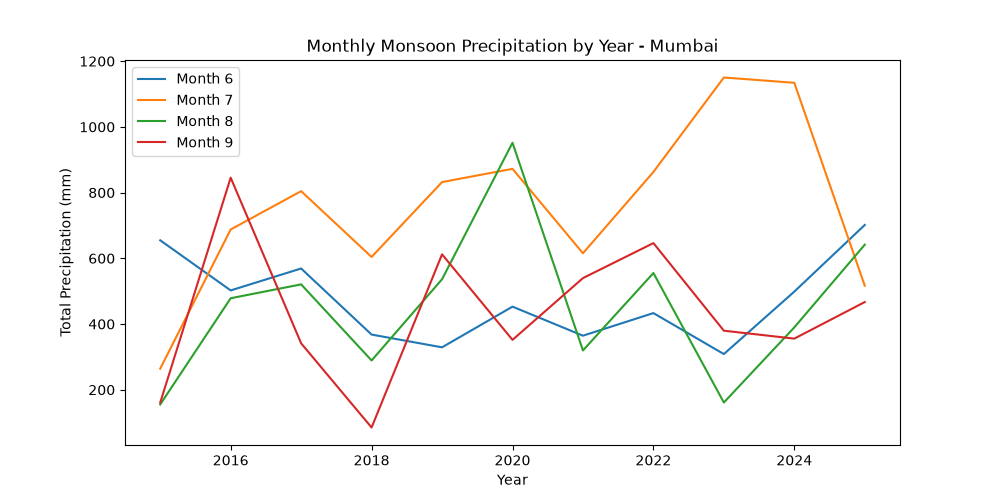
\includegraphics[width=0.8\textwidth]{monsoon_precipitation_trend.png}
\caption{Monthly monsoon-season (June--September) precipitation trend for Mumbai, 2015--2025.}
\label{fig:trend}
\end{figure}

\subsection{Feature Engineering}
Seasonal features (sine/cosine encoding of day-of-year, a monsoon-month indicator) and lagged precipitation features (previous day, previous week, 7-day rolling mean) were engineered. A chronological (non-shuffled) 80/20 train-test split was used throughout to respect the temporal structure of the data and avoid look-ahead bias.

\subsection{Models Evaluated}
Seven models were trained and compared for precipitation forecasting: Linear Regression, Random Forest, XGBoost, LightGBM (all using the engineered feature set), Prophet (date-based seasonality only), SARIMAX (ARIMA with exogenous weather variables), and an LSTM network implemented in PyTorch over 14-day input sequences (TensorFlow was found to have no available build for Python 3.14 at the time of this work, motivating the PyTorch implementation). A second target variable, next-day maximum temperature, was modeled separately using the same Random Forest approach.

\subsection{Evaluation Metrics}
Models were evaluated using Mean Absolute Error (MAE), Root Mean Squared Error (RMSE), Mean Absolute Percentage Error (MAPE, epsilon-adjusted to avoid division blow-ups on near-zero-rainfall days), and the coefficient of determination (R\textsuperscript{2}).

\subsection{Explainability}
Model interpretability was assessed using both SHAP (global feature importance via TreeExplainer) and LIME (local, per-instance explanations), applied to the Random Forest precipitation model.

\subsection{Computer Vision / Remote Sensing}
As a proof-of-concept remote-sensing component, true-color MODIS satellite imagery over Mumbai was retrieved via the NASA GIBS on-demand snapshot API for five dates spanning different seasons, and a basic OpenCV-based cloud-coverage estimator (HSV brightness/saturation thresholding) was applied and cross-referenced against recorded humidity and precipitation data.

\subsection{Generative AI Layer}
A domain-specific weather/climate knowledge base was constructed and embedded using \texttt{sentence-transformers/all-MiniLM-L6-v2}, stored in a ChromaDB vector store, and queried via a Retrieval-Augmented Generation pipeline running on a local Ollama-served open-weight LLM. A LangGraph ReAct agent was built with tools for precipitation prediction, knowledge-base search, and live-weather lookup (via Open-Meteo geocoding), extended with conversation memory (LangGraph \texttt{MemorySaver}) and a Streamlit chat interface. In addition to LangGraph's built-in tool-calling, a standalone Model Context Protocol (MCP) server and client were implemented using the official MCP Python SDK, to evaluate MCP as a standardized, protocol-level alternative to in-process LangChain tool-calling.

\section{Results}

\subsection{Precipitation Forecasting}

\begin{table}[h]
\centering
\caption{Precipitation model comparison (chronological test split)}
\begin{tabular}{lcccc}
\toprule
Model & MAE (mm) & RMSE (mm) & MAPE (\%) & R\textsuperscript{2} \\
\midrule
Linear Regression & 6.13 & 11.12 & 225.3 & 0.527 \\
Random Forest      & \textbf{3.44} & \textbf{9.30}  & \textbf{34.0}  & \textbf{0.669} \\
XGBoost            & 3.48 & 9.31  & 33.2  & 0.669 \\
LightGBM           & 3.60 & 9.30  & 34.2  & 0.669 \\
Prophet            & 5.82 & 13.66 & --    & 0.286 \\
SARIMAX            & 4.89 & 11.91 & --    & 0.457 \\
LSTM (PyTorch)     & 5.98 & 13.32 & --    & 0.317 \\
\bottomrule
\end{tabular}
\end{table}

Random Forest achieved the best overall performance. Notably, all three tree-based models (Random Forest, XGBoost, LightGBM) converge to an almost identical R\textsuperscript{2} ceiling ($\approx 0.67$), suggesting this reflects the practical limit of predictive signal available in the current feature set rather than an artifact of any single model choice. Dedicated time-series models (Prophet, SARIMAX) underperformed the feature-engineered tree models, indicating that lagged precipitation and humidity features carry more predictive signal than date-based seasonality or autoregressive structure alone. The LSTM, despite its added complexity, did not outperform Random Forest -- consistent with the well-documented finding that deep sequence models often underperform tree ensembles on small-to-moderate tabular/time-series datasets.

\subsection{Temperature Forecasting}
The Random Forest temperature model achieved MAE = 0.77\textdegree{}C, RMSE = 1.03\textdegree{}C, R\textsuperscript{2} = 0.857 -- substantially higher accuracy than the precipitation model, consistent with temperature being more day-to-day autocorrelated than rainfall.

\subsection{Explainability}
SHAP identified \texttt{precip\_lag1} (mean $|\text{SHAP}| = 6.39$) as the dominant feature, followed by relative humidity (2.38), surface pressure (0.98), maximum temperature (0.94), and wind speed (0.54). LIME, applied independently to the highest-rainfall day in the test set (actual = 136.50~mm, predicted = 73.36~mm), corroborated this ranking, with \texttt{precip\_lag1} (+14.85) and relative humidity (+10.04) as the dominant local contributors. This cross-validation across two independent explainability methods strengthens confidence in the feature importance findings. The same instance also illustrates a genuine limitation: the model under-predicted this extreme event by approximately 63~mm, consistent with tree-based models' known difficulty extrapolating to the tail of the rainfall distribution.

\begin{figure}[h]
\centering
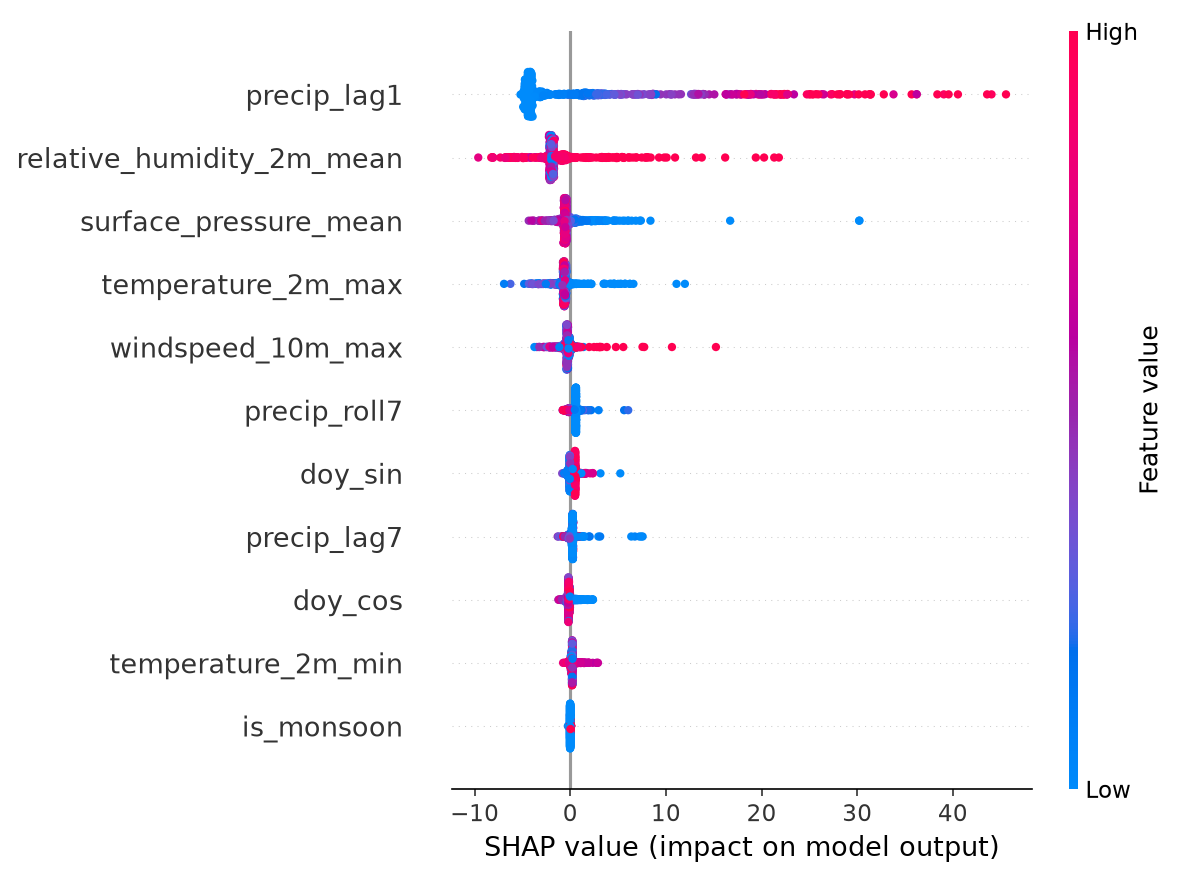
\includegraphics[width=0.85\textwidth]{shap_summary.png}
\caption{SHAP summary plot for the Random Forest precipitation model, ranking features by mean absolute SHAP value.}
\label{fig:shap}
\end{figure}

\subsection{Uncertainty Analysis}
As an approximate measure of predictive uncertainty, a prediction interval was derived from the held-out test-set RMSE of the Random Forest model (9.30~mm). Assuming approximately normally distributed residuals, this gives a rough 90\% prediction interval of $\pm 1.645 \times \text{RMSE} \approx \pm 15.3$~mm around any point forecast. This approximation, however, is known to be optimistic precisely where it matters most: as shown by the LIME case study above, errors on extreme rainfall days can exceed 60~mm, far outside this nominal interval. This indicates that residuals are not homoscedastic with respect to rainfall intensity -- the model is considerably less certain on heavy-rainfall days than on typical ones -- and that a single global prediction interval understates risk during the most operationally important events (heavy monsoon rainfall). A more rigorous treatment (e.g., quantile regression forests or conformal prediction, calibrated separately for high-rainfall regimes) is identified as future work rather than implemented here, to avoid overstating the precision of the current uncertainty estimate.

\subsection{Remote Sensing Proof of Concept}
Of five satellite imagery requests, only one (2024-07-15) returned genuine image content; the remaining four were confirmed (by file size and visual inspection) to be blank/no-data placeholder tiles from the on-demand GIBS snapshot service. For the single successful image, the OpenCV-based cloud-coverage estimate (99.99\%) aligned well with that day's recorded humidity (89\%) and monsoon-season timing. This is reported as an honest proof-of-concept rather than a systematic remote-sensing pipeline; a production version would require Google Earth Engine or a pre-downloaded Sentinel-2/MODIS archive rather than live on-demand snapshots.

\begin{figure}[h]
\centering
\includegraphics[width=0.5\textwidth]{satellite_mumbai.png}
\caption{MODIS true-color satellite image of Mumbai, 2024-07-15, retrieved via NASA GIBS.}
\label{fig:satellite}
\end{figure}

\subsection{Deployed Application}
The trained precipitation model was deployed via a FastAPI backend and a Streamlit front-end (Figure~\ref{fig:app}), allowing a user to enter current weather conditions through sliders and receive an immediate precipitation forecast alongside a color-coded risk message (light/moderate/heavy rain).

\begin{figure}[h]
\centering
\includegraphics[width=0.75\textwidth]{screenshot_ui_top.png}
\caption{Streamlit prediction application: input sliders for current weather conditions.}
\label{fig:app}
\end{figure}

\begin{figure}[h]
\centering
\includegraphics[width=0.6\textwidth]{screenshot_ui_prediction.png}
\caption{Live prediction result (4.33~mm) with the corresponding risk-tier message.}
\label{fig:app-pred}
\end{figure}

\subsection{Generative AI Layer}
The RAG pipeline retrieved relevant knowledge-base passages and produced grounded answers. Tool-calling reliability was found to differ substantially between LLM sizes: \texttt{llama3.2:1b} hallucinated fake tool-call JSON rather than invoking real LangChain/LangGraph tools, while \texttt{qwen2.5:3b} reliably triggered genuine tool calls. Even the larger model, however, was observed to selectively skip an available and relevant tool (\texttt{search\_knowledge\_base}) on at least one occasion -- documented as a real agent reliability limitation rather than silently patched. The standalone MCP server/client integration was verified end-to-end, successfully performing the full protocol handshake (\texttt{list\_tools}, \texttt{call\_tool}) and returning a correct model prediction (6.87~mm) -- demonstrating MCP as a genuinely distinct, standardized alternative to in-process LangGraph tool-calling.

\section{Discussion}
The results show that, for this dataset and feature set, simple engineered lag/seasonal features combined with tree-based ensembles outperform both dedicated time-series models and a deep sequence model, and that further gains would likely require either richer spatial/satellite features or a longer historical record rather than a more complex model architecture. The convergence of Random Forest, XGBoost, and LightGBM to the same performance ceiling is itself informative, since it rules out model choice as the current bottleneck. The explainability results (SHAP and LIME agreement) support the physical plausibility of the model: recent rainfall and humidity are meteorologically sensible short-term predictors of next-day precipitation.

\section{Limitations}
Several limitations are reported transparently. Extreme rainfall events are systematically under-predicted by all models tested. The two independent data sources (Open-Meteo, NASA POWER) show a measurable systematic offset, indicating that neither should be treated as unconditional ground truth. The remote-sensing component is a small-scale proof of concept rather than a systematic imagery pipeline, constrained by the reliability of the free on-demand satellite snapshot service used. Small open-weight LLMs are unreliable at structured tool-calling, and even a capable model can inconsistently select among available tools. Docker containerization, while fully specified (\texttt{Dockerfile}, \texttt{requirements.txt}), could not be verified end-to-end due to a persistent Windows-level WSL2/DISM installation issue on the development machine, unrelated to the application code itself. No k-fold cross-validation was performed; all reported metrics use a single chronological train-test split.

\section{Conclusion and Future Work}
This work demonstrates a complete, reproducible, open-source pipeline for Southwest Monsoon precipitation forecasting, from data acquisition through explainable machine learning to a deployed Generative AI assistant with genuine RAG, agentic tool-calling, and MCP integration. Future work includes completing Docker containerization, extending the remote-sensing component with a systematic Sentinel-2/Earth Engine pipeline and a trained CNN classifier, incorporating k-fold cross-validation, and expanding the knowledge base with additional peer-reviewed monsoon literature.

\section*{Acknowledgements}
This work was completed as part of the Phase 02 Generative AI Research Internship at MacroEdtech, under the guidance of Sagar Sakalley.

\begin{thebibliography}{9}

\bibitem{kumar2025ann}
A. Kumar, S. Singh, A. Malik, and Manju, ``Forecasting of Southwest Indian Summer Monsoon Rainfall Using Artificial Neural Networks,'' \textit{National Academy Science Letters}, 2025. DOI: \url{10.1007/s40009-025-01862-5}.

\bibitem{dash2018comparison}
Y. Dash, S. K. Mishra, S. Sahany, and B. K. Panigrahi, ``Indian summer monsoon rainfall prediction: a comparison of iterative and non-iterative approaches,'' \textit{Applied Soft Computing}, vol. 70, pp. 1122--1134, 2018. DOI: \url{10.1016/j.asoc.2017.08.055}.

\bibitem{hochreiter1997lstm}
S. Hochreiter and J. Schmidhuber, ``Long Short-Term Memory,'' \textit{Neural Computation}, vol. 9, no. 8, pp. 1735--1780, 1997.

\bibitem{lundberg2017shap}
S. M. Lundberg and S.-I. Lee, ``A Unified Approach to Interpreting Model Predictions,'' \textit{Advances in Neural Information Processing Systems (NeurIPS)}, 2017.

\bibitem{ribeiro2016lime}
M. T. Ribeiro, S. Singh, and C. Guestrin, ``Why Should I Trust You? Explaining the Predictions of Any Classifier,'' \textit{Proceedings of the 22nd ACM SIGKDD International Conference on Knowledge Discovery and Data Mining}, pp. 1135--1144, 2016.

\bibitem{gao2023rag}
Y. Gao, Y. Xiong, X. Gao, K. Jia, J. Pan, Y. Bi, Y. Dai, J. Sun, M. Wang, and H. Wang, ``Retrieval-Augmented Generation for Large Language Models: A Survey,'' \textit{arXiv preprint arXiv:2312.10997}, 2023.

\bibitem{langgraph2024}
LangChain AI, ``LangGraph: Build resilient language agents as graphs,'' Documentation, \url{https://langchain-ai.github.io/langgraph/}, accessed 2026.

\bibitem{mcp2024}
Anthropic, ``Model Context Protocol Specification,'' \url{https://modelcontextprotocol.io}, accessed 2026.

\end{thebibliography}

\end{document}